\documentclass{article}
\usepackage{ae,aecompl}
\usepackage{todonotes}
\usepackage{chngcntr}
\usepackage{tikz-cd}
\usepackage{graphicx}
\graphicspath{ {./images/}}
\usepackage[all,cmtip]{xy}
\usepackage{amsmath, amscd}
\usepackage{amsthm}
\usepackage{amssymb}
\usepackage{amsfonts}
\usepackage{bm}
\usepackage{qsymbols}
\usepackage{latexsym}
\usepackage{mathrsfs}
\usepackage{mathtools}
\usepackage{cite}
\usepackage{color}
\usepackage{url}
\usepackage{enumerate}
\usepackage{verbatim}
\usepackage[draft=false, colorlinks=true]{hyperref}
\usepackage{pdfpages}
\usepackage[margin=1.2in]{geometry}
\usepackage{IEEEtrantools}

\usepackage{fancyhdr}


\usepackage[nameinlink]{cleveref}


\DeclareMathOperator*{\ac}{accept}
\DeclareMathOperator*{\amax}{argmax}
\DeclareMathOperator*{\amin}{argmin}
\DeclareMathOperator*{\Aut}{Aut}
\newcommand {\al}{{\alpha}}
\newcommand {\abs}[1]{{\left\lvert#1\right\rvert}}
\newcommand {\A}{{\mathcal{A}}}
\newcommand {\AM}{{\mathrm{AM}}}
\newcommand {\AMp}{{\AM_{p}^{X}\!(\Ri_\w)}}
\newcommand {\B}{{\mathcal{B}}}
\DeclareMathOperator*{\Be}{Bern}
\newcommand {\Br}{{\dot{B}}}
\newcommand {\Ba}{{\mathfrak{B}}}
\newcommand {\C}{{\mathbb C}}
\newcommand {\ce}{\mathrm{c}}
\newcommand {\Ce}{\mathrm{C}}
\newcommand {\Cc}{\mathrm{C_{c}}}
\newcommand {\Ccinf}{\mathrm{C_{c}^{\infty}}}
\DeclareMathOperator{\cov}{Cov}
\DeclareMathOperator{\DEV}{DEV}
\newcommand {\Di}{{\mathbb D}}
\newcommand {\dom}{\mathrm{dom}}
\newcommand{\dist}{\stackrel{\mathrm{dist}}{=}}
\newcommand {\ud}{\mathrm{d}}
\newcommand {\ue}{\mathrm{e}}
\newcommand {\eps}{\varepsilon}
\newcommand {\veps}{\varepsilon}
\newcommand {\vrho}{{\varrho}}
\newcommand {\E}{{\mathbb{E}}}
\newcommand {\Ec}{{\mathcal{E}}}
\newcommand {\Ell}{L}
\newcommand {\Ellp}{{L_{p}[0,1]}}
\newcommand {\Ellpprime}{{L_{p'}([0,1])}}
\newcommand {\Ellq}{{L_{q}([0,1])}}
\newcommand {\Ellqprime}{{L_{q'}([0,1])}}
\newcommand {\Ellr}{L^{r}}
\newcommand {\Ellone}{{L_{1}([0,1])}}
\newcommand{\Elltwo}{{L_{2}([0,1])}}
\newcommand{\Ellinfty}{L^{\infty}}
\newcommand{\Ellinftyc}{L_{\mathrm{c}}^{\infty}}
\newcommand{\exb}[1]{\exp\left\{#1\right\}}
\DeclareMathOperator*{\Ext}{Ext}
\newcommand{\F}{{\mathcal{F}}}
\newcommand{\Fe}{{\mathbb{F}}}
\newcommand{\G}{{\mathcal{G}}}
\newcommand{\HF}{\mathcal{H}_{\text{FIO}}^{1}(\Rd)}
\newcommand{\Hr}{H}
\newcommand{\HT}{\mathcal{H}}
\newcommand{\ui}{\mathrm{i}}
\newcommand{\I}{{I}}
\newcommand{\J}{{\mathcal{J}}}
\newcommand{\id}{{\mathrm{id}}}
\newcommand{\iid}{\stackrel{\mathclap{\normalfont\mbox{iid}}}{\sim}}
\newcommand{\im}{{\text{im }}}
\newcommand{\ind}{{\perp\!\!\!\perp}}
\DeclareMathOperator*{\Int}{int}
\newcommand{\intx}{{\overline{\int_{X}}}}
\newcommand{\inte}{{\overline{\int_{\E}}}}
\newcommand{\la}{\lambda}
\newcommand{\rb}{\rangle}
\newcommand{\lb}{{\langle}}
\newcommand{\La}{\Lambda}
\newcommand{\calL}{{\mathcal{L}}}
\newcommand{\lp}{{\mathcal{L}}^{p}}
\newcommand{\lpo}{{\overline{\mathcal{L}}^{p}\!}}
\newcommand{\Lpo}{{\overline{\Ell}^{p}\!}}
\newcommand{\M}{{\mathbf{M}}}
\newcommand{\Ma}{{\mathcal{M}}}
\newcommand{\N}{{{\mathbb N}}}
\newcommand{\Na}{{{\mathcal{N}}}}
\newcommand{\norm}[1]{\left\|#1\right\|}
\newcommand{\normm}[1]{{\left\vert\kern-0.25ex\left\vert\kern-0.25ex\left\vert #1 
    \right\vert\kern-0.25ex\right\vert\kern-0.25ex\right\vert}}
\newcommand{\Om}{{{\Omega}}}
\newcommand{\one}{{{\bf 1}}}
\newcommand{\pic}{\text{Pic }}
\newcommand{\ph}{{\varphi}}
\newcommand{\Pa}{{\mathbb{P}}}
\newcommand{\Po}{{\mathcal{P}}}
\newcommand{\Q}{{\mathbb{Q}}}
\newcommand{\R}{{\mathbb R}}
\newcommand{\Rd}{{\mathbb{R}^{d}}}
\DeclareMathOperator{\rej}{reject }
\newcommand{\Rn}{{\mathbb{R}^{n}}}
\newcommand{\cR}{{\mathcal{R}}}
\newcommand{\Rad}{{\mathrm{Rad}}}
\newcommand{\ran}{{\mathrm{ran}}}
\newcommand{\Ri}{{\mathrm{R}}}
\newcommand{\supp}{{\mathrm{supp}}}
\newcommand{\Se}{\mathrm{S}}
\newcommand{\Sp}{S^{*}(\Rn)}
\newcommand{\St}{{\mathrm{St}}}
\newcommand{\Sw}{\mathcal{S}}
\newcommand{\T}{{\mathcal{T}}}
\newcommand{\ta}{{\theta}}
\newcommand{\Ta}{{\Theta}}
\newcommand{\topp}{\stackrel{p}{\to}}
\newcommand{\todd}{\stackrel{d}{\to}}
\newcommand{\toL}[1]{\stackrel{L^{#1}}{\to}} 
\newcommand{\toas}{\stackrel{a.s.}{\to}}
\DeclareMathOperator{\V}{Var}
\newcommand {\w}{{\omega}}
\newcommand {\W}{{\mathrm{W}}}
\newcommand {\Wnp}{\text{$\mathrm{W}$\textsuperscript{$n,\!p$}}}
\newcommand {\Wnpeq}{\text{$\mathrm{W}$\textsuperscript{$n\!,\!p$}}}
\newcommand {\Wonep}{\text{$\mathrm{W}$\textsuperscript{$1,\!p$}}}
\newcommand {\Wonepeq}{\text{$\mathrm{W}$\textsuperscript{$1\!,\!p$}}}
\newcommand {\X}{{\mathcal{X}}}
\newcommand {\Z}{{{\mathbb Z}}}
\newcommand {\Za}{{\mathcal{Z}}}
\newcommand {\Zd}{{\Z[\sqrt{d}]}}
\newcommand {\vanish}[1]{\relax}

\newcommand {\wh}{\widehat}
\newcommand {\wt}{\widetilde}
\newcommand {\red}{\color{red}}

% Distributions
\newcommand{\normal}{\mathsf{N}}
\newcommand{\poi}{\mathsf{Poisson}}
\newcommand{\bern}{\mathsf{Bernoulli}}
\newcommand{\bin}{\mathsf{Binomal}}
\newcommand{\multi}{\mathsf{Multinomial}}
\newcommand{\Exp}{\mathsf{Exp}}



% put your command and environment definitions here




% some theorem environments
% remove "[theorem]" if you do not want them to use the same number sequence


  \newtheorem{thrm}{Theorem}
  \newtheorem{lemma}{Lemma}
  \newtheorem{prop}{Proposition}
  \newtheorem{cor}{Corollary}

  \newtheorem{conj}{Conjecture}
  \renewcommand{\theconj}{\Alph{conj}}  % numbered A, B, C etc

  \theoremstyle{definition}
  \newtheorem{defn}{Definition}
  \newtheorem{ex}{Example}
  \newtheorem{exs}{Examples}
  \newtheorem{question}{Question}
  \newtheorem{remark}{Remark}
  \newtheorem{notn}{Notation}
  \newtheorem{exer}{Exercise}




\title{STATS305A - Lecture 7}
\author{John Duchi\\ Scribed by Michael Howes}
\date{10/12/21}

\pagestyle{fancy}
\fancyhf{}
\rhead{STATS305A - Lecture 7}
\lhead{10/12/21}
\rfoot{Page \thepage}

\begin{document}
\maketitle
\tableofcontents

\section{Announcements}
\begin{itemize}
    \item Etude 1 due 5pm Thursday sharp
    \begin{itemize}
        \item On Thursday solutions to the etude will be posted at around 5pm.
        \item Students grade their own etudes.
        \item Students upload a new etude with corrections made to the orginal submission. You must upload a revised etude. This second submission is due 5pm Friday.
    \end{itemize}
    \item Homework 2 will be out soon.
\end{itemize}

\section{Fisherian Testing}
\subsection{Setting} 

We propose a null $H_0$. We collect data and compute a statistic $T_n$ which is just some function of our data. Under the null $H_0$, $T_n$ follows \emph{some} distribution. Call this distribution $T$ (this is not a $T$-distribution, just the distribution of $T_n$ when the null holds).

We nest pick a \emph{level} $\al \in (0,1)$ at which to reject $H_0$. We choose a \emph{rejection region} $R$ where 
\[\Pa_{H_0}(T \in R) \le \al. \]
That is, under the null $H_0$, $T_n$ is unlikely to fall in $R$. We then reject if $T_n \in R$.

\subsection{P-values}
Often our rejection regions are nested. That is if $R_{\al}$ denotes the rejection region at level $\al$, then 
\[R_{\al_0} \subsetneqq R_{\al_1}, \text{ if } \al_0 < \al_1. \]

For example if $T \sim \Na(0,1)$ under $H_0$, then we often choose
\[R_{\al} = (-\infty, -z_{1-\al/2}) \cup (z_{1+\al/2},\infty),\]
where $z_{1-\al}$ is the $1-\al$ quantile of a standard normal $Z \sim \Na(0,1)$, that is $\Pa(Z \ge z_{1-\al}) = \al$. See below
\begin{center}
    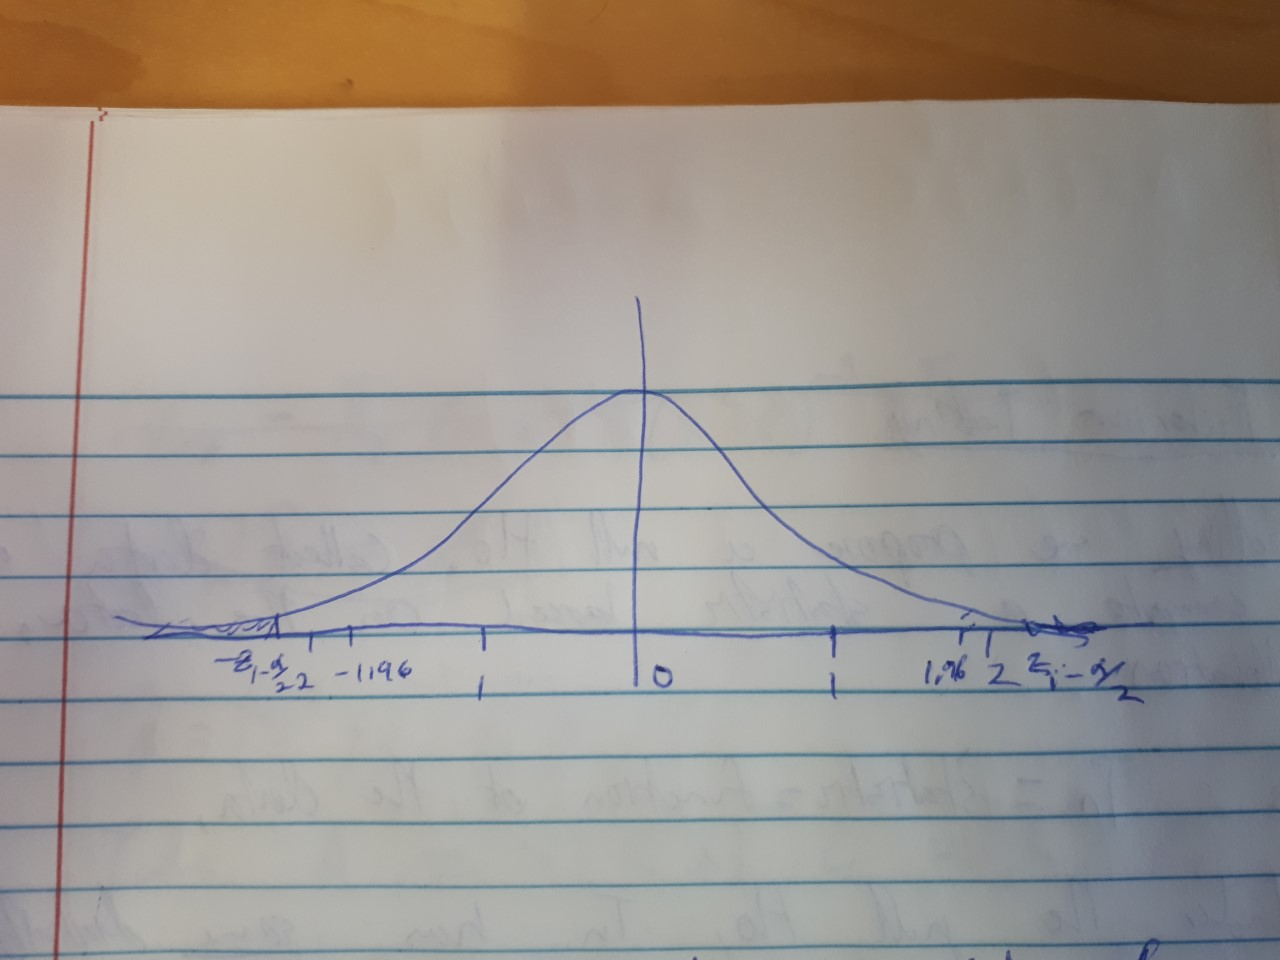
\includegraphics[width = \textwidth/2]{10_12_P01.jpg}
\end{center}

The \emph{p-value} of a statistic $T_n$ is:
\begin{itemize}
    \item The smallest level $\al$ at which we can reject the test ie $p = \inf\{\al : T_n \in R_{\al}\}$.
    \item Equivalently, the probability under $H_0$ of seeing a sample as strange/extreme as what we have observed.
\end{itemize}
\begin{ex}
Consider the example above when $H_0$ implies that $T_n$ is normally distributed. Set $t_n := T_n$ (the observed value), then our p-value is 
\[p = \Pa_{H_0}(\abs{T} \ge \abs{T_n}). \]
\end{ex}
\begin{ex}
    Assume that $Y = X\beta + \one \beta_0 + \eps$ where $X \in \R^{n \times (d-1)}$ and $Z = [1, X]$. Let $H = Z(Z^TZ)^{-1}Z = $ projection onto full model. Let $H_0 = \frac{1}{n}\one \one^T = $ projection onto range of the submodel $Y = \one \beta_0 + \eps$. Our null hypothesis is that the submodel is true. Define $S_n^2 = \frac{1}{n-d}\norm{(I-H)Y}_2^2$. Under the null hypothesis we saw that
    \[T_n := \frac{\frac{1}{d-1}\norm{(H-H_0)Y}_2^2}{\frac{1}{n-d}\norm{(I-H)Y}_2^2} \sim F_{d-1, n-d}. \]
    We reject the null if $T_n$ is large which means the larger model explains the data better than the smaller model.
\end{ex}
\subsection{Sampling/M-tests}
Suppose that we decide to estimate $\beta$ via 

\[\wh{\beta} = \arg\min_b \sum_{i=1}^n \abs{Y_i-X_i^Tb}. \]
Where we assume $Y = X\beta + \varepsilon$, $\varepsilon \sim \Na(0,\sigma^2 I)$ where we assume $\sigma^2$ is known. We wish to test the null hypothesis $\beta = 0$.

Under the null hypothesis we can compute $\eps^{(1)}, \ldots, \eps^{(N)}$ independent samples from $\Na(0, \sigma^2 I)$ where $N$ is big. We then define $Y^{(i)} := \eps^{(i)}$ and
\[\wh{\beta}^{(i)} = \arg\min_b \sum_{j=1}^n \abs{Y_j^{(i)} - X_jb}. \]
The samples $\wh{\beta}^{(i)}$ gives us an approximation to the distribution of $\wh{\beta}$ assuming that the null is true. 

Abstractly all we need is some region in $\R^d$ that contians a $1-\al$ fraction of all $\wh{\beta}^{(i)}$. Then we reject the null if $\wh{\beta}$ is out of that region. Here is one way to do this.

We could compute $q_{1-\al}^{sim} = 1-\al$ quartile of $\norm{\wh{\beta}^{(i)}}_2$. Thus we have 
\[\Pa_{H_0}\left(\norm{\wh{\beta}} \ge q_{1-\al}^{sim}\right) \le \al + \frac{1}{N}. \]
This is because under $H_0$, $\norm{\wh{\beta}^{(i)}}_2$ has the same distribution as $\norm{\wh{\beta}}$. If we define $t_i = \norm{\wh{\beta}^{(i)}}_2$ and $T_n = \norm{\wh{\beta}}_2$, then $\norm{\wh{\beta}}_2 > q_{1-\al}^{sim}$ if and only if $T_n > t_i$ for a $1-\al$ fraction of $\{t_1,\ldots, t_n\}$. And $T_n > t_i$ for a $1-\al$ fraction of $\{t_1,\ldots, t_n\}$ occurs with probability $\al \pm \frac{1}{N}$. 

The p-value in this case is
\begin{IEEEeqnarray*}{rCl}
    &&\inf\{\al : \norm{\wh{\beta}}_2 > t_i \text{ for a } 1-\al \text{ fraction of } \{t_i\}_{i=1}^N\}\\
    &=&\inf\{ \al : \norm{\wh{\beta}}_2 > q^{sim}_{1-\al}\}\\
    &\approx& \text{the fraction of } \{t_i\}_{i=1}^N \text{ such that } \norm{\wh{\beta}}_2 \le t_i.
\end{IEEEeqnarray*}

\subsection{Aside: power of a test}
Choose an alternative $H_1$ such as $Y=X\beta + \varepsilon$, $\norm{\beta} \ge \sqrt{\frac{d}{n}}$ or $Y=X\beta+\varepsilon$, $\beta_1 > \frac{1}{\sqrt{n}}$. 

The \emph{power} of a test is also written as $\beta$ but now $\beta$ is a probability not a parameter in a model. The power is defined as
\[\beta := \Pa_{H_1}(T_n \text{ rejects}). \]
Once could try to maximise the power of a test while keeping the level $\al$ constant but this is subtle and complicated. The rejection region with the most power will depend on $H_1$. More often in practice we focus on the level and choose the rejection region in a way that reflects the null/alternative hypotheses.

\section{ANOVA (Analysis of variance)}
Suppose we have the model
\[Y_{ij}= \mu + \al_i + \varepsilon_{ij},\]
where $i=1,\ldots,k$ are different groups and $Y_{i,j}$ for $j=1,\ldots, n_i$ are different samples from group $i$. We call $\mu$ the population mean and $\al_i$ the group effect. We are interested in testing/estimating the differences $\al_i - \al_{j}$. The structure of this model allows us to write cleaner/more direct computations and tests.

\subsection{ANOVA Decomposition}
Let $\overline{Y}_{\bullet\bullet} = \frac{1}{N}\sum_{i=1}^k \sum_{j=1}^{n_i}Y_{i,j}$ be the global mean ($N = n_1+n_2+\ldots+n_k$). Let $\overline{Y}_{i\bullet} = \frac{1}{n_i}\sum_{j=1}^{n_i} Y_{ij}$ be the mean for group $i$. Define
\begin{IEEEeqnarray*}{rCl}
    SST&:=& \sum_{i=1}^k \sum_{j=1}^{n_i} \left(Y_{i,j}-\overline{Y}_{\bullet \bullet}\right)^2 \quad (\text{total sum of squares.})\\
    SSB&:=& \sum_{i=1}^k \sum_{j=1}^{n_i} \left(\overline{Y}_{i\bullet}-\overline{Y}_{\bullet \bullet}\right)^2 \quad (\text{between groups sum of squares.})\\
    &=&\sum_{i=1}^k n_i \left(\overline{Y}_{i\bullet}-\overline{Y}_{\bullet \bullet}\right)^2 \\
    SSW&:=& \sum_{i=1}^k \sum_{j=1}^{n_i} \left(Y_{i,j}-\overline{Y}_{i \bullet}\right)^2 \quad (\text{within groups sum of squares.})
\end{IEEEeqnarray*} 
We then have
\begin{IEEEeqnarray*}{rCl}
    SST &=&\sum_{i=1}^k \sum_{j=1}^{n_i} \left(Y_{i,j}-\overline{Y}_{\bullet \bullet}\right)^2\\
    &=&\sum_{i=1}^k \sum_{j=1}^{n_i} \left(Y_{i,j}-\overline{Y}_{i \bullet}+\overline{Y}_{i \bullet}-\overline{Y}_{\bullet \bullet}\right)^2\\
    &=&\sum_{i=1}^k \sum_{j=1}^{n_i} \left(Y_{i,j}-\overline{Y}_{i \bullet}\right)^2+\sum_{i=1}^k \sum_{j=1}^{n_i} \left(\overline{Y}_{i\bullet}-\overline{Y}_{\bullet \bullet}\right)^2\\
    &=&\sum_{i=1}^k \sum_{j=1}^{n_i} \left(Y_{i,j}-\overline{Y}_{i \bullet}\right)^2+\sum_{i=1}^k \sum_{j=1}^{n_i} \left(\overline{Y}_{i\bullet}-\overline{Y}_{\bullet \bullet}\right)^2\\
    &=&SSW+SSB
\end{IEEEeqnarray*}
This is called the ANOVA decomposition. 

Suppose our null is $H_0:\al_1=\al_2=\ldots =\al_k=0$, $\eps_{i,j} \sim \Na(0,\sigma^2)$. Then (exercise) under $H_0$:
\begin{itemize}
    \item $SSW \ind SSB.$
    \item $SSW \sim \sigma^2 \chi^2_{N-k}$.
    \item $SSB \sim \sigma^2 \chi^2_{k-1}$.
\end{itemize}
Thus $\frac{{1}{k-1}SSB}{\frac{1}{N-k}SSW} \sim F_{k-1, N-k}$.

We reject $H_0$ when the above statistic is large which means the between group differences are large relative to the within-group differences. 

\subsection{Testing differences}
Often we may care more about differences in between the mean treatments. For example we may be dosing a drug at different levels $i=1,\ldots, k$. We care more about $\al_i -\al_j$ more than just ``is there a difference in treament from $\al_1=\al_2=\ldots=\al_k=0$?'' 

This gives rise to testing \emph{constrasts} which are vectors $c \in \R^k$ satisfying $c^T \one = 0$. For example $c = e_i - e_j$. If $\wh{\al}$ is any least squares solution then $\frac{c^T \wh{\al}}{S\sqrt{c^T(X^TX)^\dagger c}} \sim T_{n-(d-1)}$ ($T$-distribution), where $S^2 = \frac{1}{n-(d-1)}\sum_{i=1}^n (Y_i-X_i^T\wh{\beta})^2$. 

Exercise: If $c = e_i -e_j$ (ie $c^T \beta = \al_i -\al_j$), then $c^T(X^TX)^\dagger c = \frac{1}{n_i}+\frac{1}{n_j}$. 

\subsection{An issue}
If we look at all pairs of differences $\al_i -\al_j$ for $i< j$. Then we are doing $\frac{k(k-1)}{2}$ tests. If we reject the nulls at a level $\al$, then we ``expect'' to have roughly $\al \frac{k^2}{2}$ false rejections. Note that $\al \frac{k^2}{2} >> \al$. This is the issue of \emph{multiple testing}.
\end{document}